\cleardoublepage
\chapter{CHOPs}
\label{ch:4}

%------------------------------------------------

\section{Introduction}

\begin{fullwidth}
The Channel Operators, or CHOP, family of Operators handle all channel operations including motion data, audio inputs, key-frame animations, hardware inputs (from Microsoft Kinect, Leap Motion, Oculus Rift, pen tablets, keyboards, mice, etc), DMX, MIDI, and OSC. These are the Operators that handle inputs, processing, and outputs, of the data used to communicate with many types of audio-visual gear such as:

\begin{itemize}
\item Mixers
\item MIDI controllers
\item Synths
\item DMX lighting fixtures
\item Microsoft Kinect cameras
\item Computers running TouchDesigner
\item Loudspeakers
\item Other audio-video application like Max/MSP, Ableton Live, Resolume Arena
\end{itemize}

\end{fullwidth}

%------------------------------------------------

\section{Communication Methods}

\begin{fullwidth}
MIDI works with an extensive amount of existing software and hardware. Digital Audio Workstations, or DAWs, like Ableton Live, Avid Pro Tools, Propellerhead Reason, and more, all support MIDI input and output. It is a relatively fast, stable, and time-tested protocol. Audio performance controllers often comes equipped with MIDI over USB. These controllers include inputs hardware with controls such as: buttons, faders, piano keys, touch strips, jog wheels, drum pads, and potentiometers.

Programming environments such as Cycling 74 Max/MSP, PureData, Native Instruments Reaktor, and more, have support for OSC messaging. OSC messaging has the benefit of modern networking technology, higher resolutions than MIDI, channel naming, and many structural improvements. OSC messaging can be sent over UDP or TCP connections, making it incredibly easy to network, and transmit long distances in real-time. Currently, OSC is more commonly used as a communication method between softwares and computer systems.

DMX is a protocol used by lighting fixtures and controllers. Many DMX fixtures have various channels for dimmers, various settings, built-in chases, RGB channels, motor automation, and more. Many lighting controllers and desks use DMX protocol to communicate with fixtures and video-computer systems. With the many types of controllers and desks available, their manuals will be invaluable when creating projects with them in mind. In general, all of a fixtures channels need to be accounted for, even if aren't being actively used. There are many ways to optimize the workflow of sending and receiving DMX data, mostly concerning the management and organization of channels. These will be looked at in later examples.

Sync In CHOP and Sync Out CHOP are used to frame sync internal and external instances of TouchDesigner. They use the OSC protocol for their underlying communication. These two Operators work by communicating the state of each frame on every synced machine. Once all sync machines confirm that they have rendered the current frame, they simultaneously move to the next frame. This sequence of events is repeated for every frame and keeps the synced machines always on the same frame. 
\end{fullwidth}

%------------------------------------------------

\section{Audio Inputs and Outputs}

\begin{fullwidth}
Audio can be processed from a variety of sources, and can be processed in a variety of ways. TouchDesigner is capable of processing audio from audio files, movie files, external audio interfaces, internet audio streams, and can even synthesize audio from nothing. 

Most projects involving sound design and audio tracks will include dedicated audio files. TouchDesigner is capable of reading and playing many standard audio formats such as MP3, AIFF, and WAV, through the use of the Audio File In CHOP and the Audio Play CHOP. These files can be looped, cued, re-pitched, and trimmed, allowing for flexible uses of samples and audio files.

The Audio Movie CHOP can be used to playback audio from a movie file. Instead of reading audio by referencing a file, this CHOP references a Movie In TOP. This is useful because it keeps the audio in sync with the video playing back in the Movie In TOP, and comes with a parameter that can be used to offset the audio to better match the video.

There are many different external audio interfaces that can be used with TouchDesigner. It is best to refer to the Derivative TouchDesigner Wiki and Forum for a more comprehensive list of compatible devices. 

These devices provide analog and digital audio inputs and outputs. These can be inputs from musicians and instrumentalists, audio mixing consoles, professional video cameras, other computer systems, and much more. These devices can output audio to many of the above mentioned destinations, as well as to loud speaker systems. The CHOPs used to communicate with external interfaces are the Audio Device In CHOP and the Audio Device Out CHOP. Each respectively handles the inputs and outputs, to and from, a project. There is an Audio SDI CHOP which is used in conjunction with the nVidia Quadro SDI card, to receive audio from external SDI sources. 

There are two different audio drivers that can be accessed from within TouchDesigner. DirectSound has been available since previous versions of TouchDesigner, and has been developed as a part of DirectX. It is a mature driver, having been in development for many years, and provides relatively low latencies even under heavy use. 

ASIO is a new addition to TouchDesigner 088. It has been developed by Steinberg to improve on one of DirectX's main drawbacks, which is that DirectX feeds all audio through the Windows operating system. Bypassing the operating system, the ASIO driver is able to communicate directly with external audio hardware, thus creating lower latencies than what was previously possible with DirectSound.

Once inputs and outputs are setup in TouchDesigner, they can be routed much like any other data. 

\end{fullwidth}

%------------------------------------------------

\section{Sample Rates}

\begin{fullwidth}
Many applications never expose the granular functions and operations that are happening behind the scenes. Because of this, many people aren't used to processing audio in a mathematical fashion. Audio is, at its core, numerical data being processed incredibly fast. Knowing this lays the groundwork for how to work with audio in TouchDesigner. 

Open up example 'Sample\_rates\_1.toe'. This example creates a very basic feature common in many audio applications: muting. This is achieved by using a Math CHOP to multiply the audio stream by the output value of a Button COMP, which is either 0 or 1. Like any other mathematical equation, a value, in this case each sample of audio, multiplied by 0 will always be 0. Similarly, a value, or audio sample, multiplied by 1 will be returned unchanged. These two states produce on and off states for this audio example.  

Let's take this example a step further by allowing the button to fade the audio in and out. Open example 'Sample\_rates\_2.toe'. 

This example takes the previous example and adds two Operators. The first is the Filter CHOP which smoothens the input value. This creates a smooth ramp between the two states of the button. The second is a Resample CHOP. 

The sample rate of different Operators is something that is overlooked by many beginners, but is essential to having artifact-free audio. The Oscillator CHOP is being sampled 44,100 times a second, and the Filter CHOP is being sampled 60 times a second. This discrepancy means that there will not be a 1:1 ratio between the samples of audio and the samples of the ramp when they are multiplied. More accurately, there will be a 735:1 ratio between samples of audio and samples of the ramp. This means when the two values are multiplied, the audio will step up or down in volume every 735 samples. Examine the diagram below, where the dotted blue line is a 1:1 ratio, and the dotted red line represents a 735:1 ratio.

\begin{center}
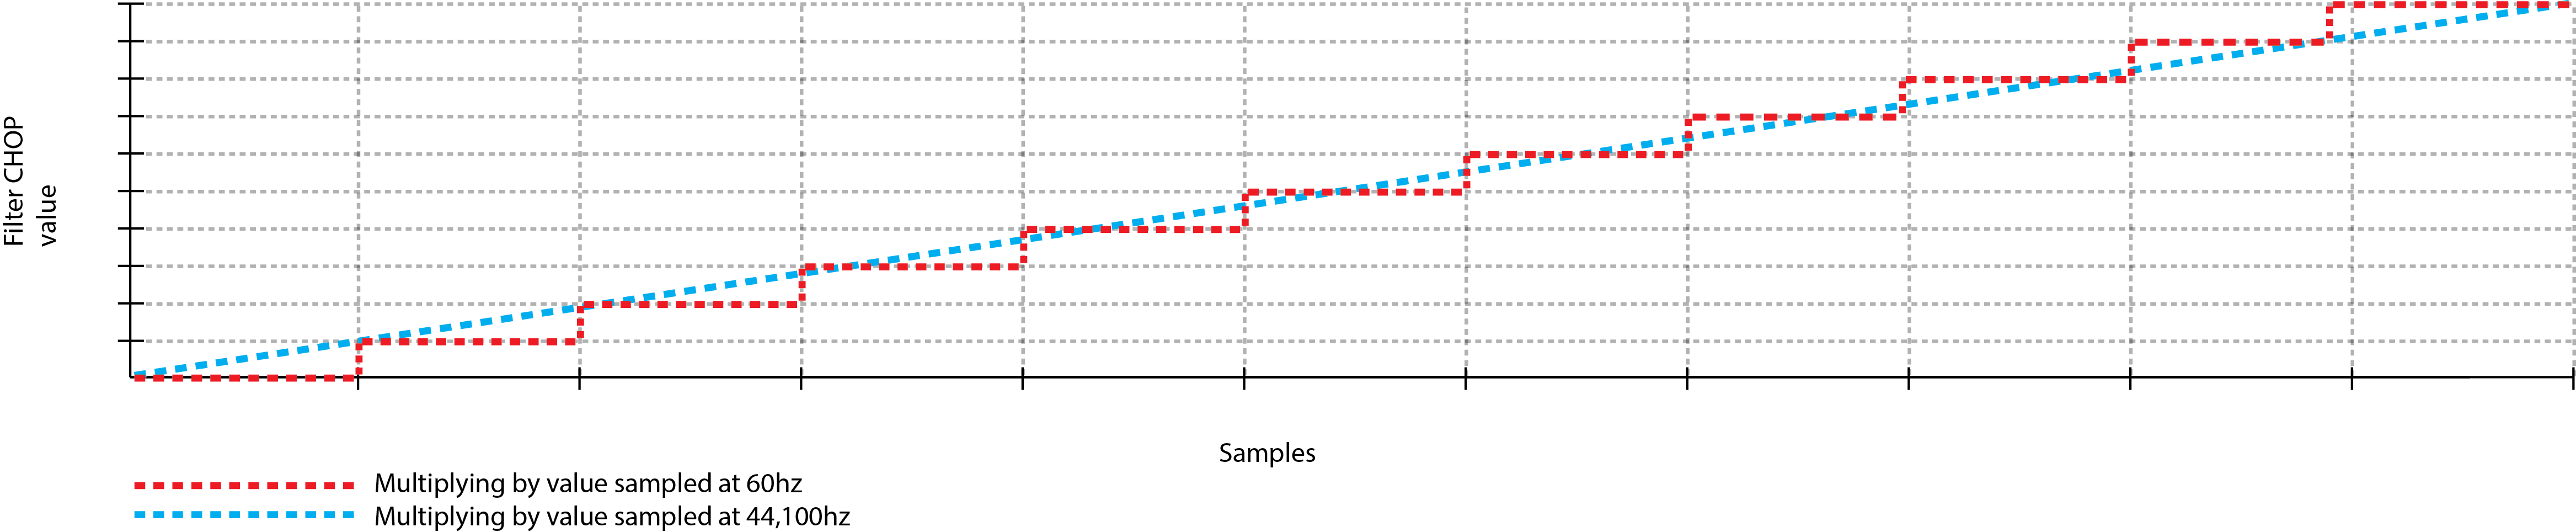
\includegraphics{./img/4.4/sample-rate.png}
\end{center}

Looking at the diagram above, there is a very distinct stepping that happens when the two channels that have different sample rates are multiplied. Many CHOPs use the project FPS as their default sample rate, causing the stepping to become exaggerated when the project is set to run at 30 FPS. Using the same example as above, the ratio of samples of audio and samples of the ramp would jump from 735:1 to 1470:1. This means in a 30 FPS project, there would only be an incremental volume change every 1470 samples! 

The above examples highlight the need to always be aware of the sample rates of CHOPs in a project, and to use the Resample CHOP when necessary. Many times, this situation will occur in regards to audio, but there are instances where control data might need to be input or output at a different sample rate. 

\end{fullwidth}

%------------------------------------------------
\section{Time Slicing}

\begin{fullwidth}

Time slicing is something that is unique to TouchDesigner, and can be a bit tricky to understand at first. 

A Time slice is the period between the last rendered frame and the current rendered frame. Think of Time slices as dynamic amounts of time. If a project is running at a consistent 60 FPS, then the time slices will be 1 frame in length. If a project is having trouble keeping up with real-time, and drops 10 frames, the corresponding time slice would be 10 frames in length.

Time slicing exists to smoothen out CHOP data in situations where frames are dropped. To think about it simply, Time slicing is when CHOPs start taking the size of Time slices into account when cooking. Think of this as a kind of adaptive cooking, meaning that as the time slices grow in length, the CHOPs will compensate for the amount of frames lost, and cook the amount of frames necessary to produce smoother outputs. This is in contrast to CHOPs that aren't time sliced, that will cook their value at the last cooked frame, then jump to the value at the next cooked frame, no matter how many frames are dropped inbetween. Only CHOPs can take advantage of Time slicing.

Using the example above, when the timeline is running consistently at 30 FPS, every time slice is 1 frame in length. If there are two ramps going from 0 to 1 over the course of one second (30 frames), both outputs would be smooth ramps. If, for some bizarre reason, only every tenth frame was cooked, there would be very different results. In the non-time sliced CHOP, the value would jump every time a frame is cooked, while the data between those cooked frames is lost. The Time sliced CHOP is aware that it is only being cooked every tenth frame, and will cook the frames inbetween to interpolate between the value of the last cooked frame, and the current cooked frame. This keeps the data smooth no matter what is going on. 

The diagram below illustrates the above example, where the dotted-blue line is a non-Time sliced CHOP, the dotted-red line is a Time sliced CHOP, and the vertical dotted-green lines represent a cooked frame: 

\begin{center}
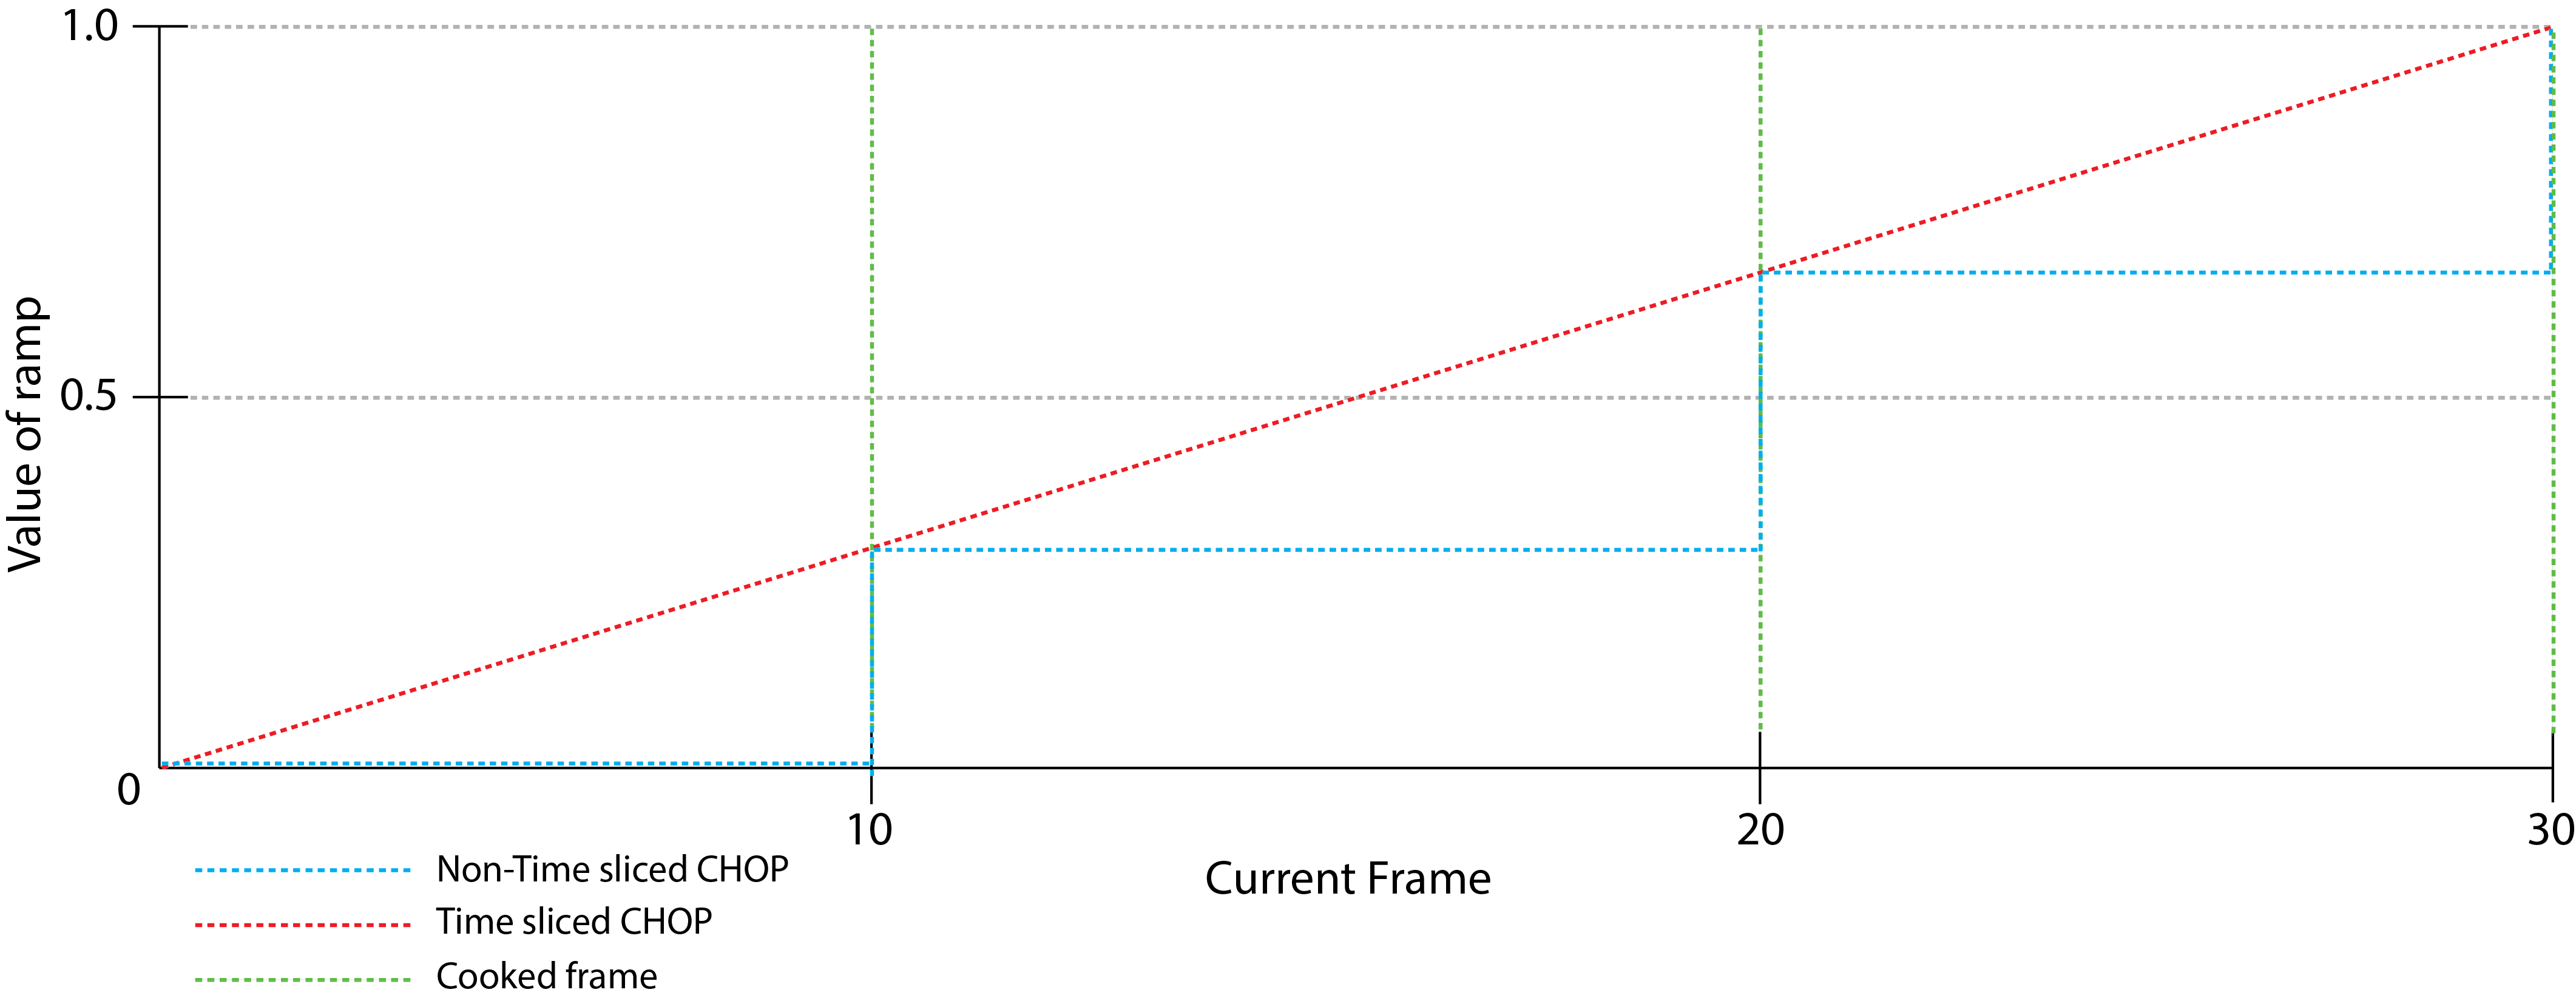
\includegraphics[width=14cm]{./img/4.4/Timeslice.png}
\end{center}

\end{fullwidth}
